\chapter{Introduction au calcul des cartes de reionisation}


Les cartes de redshift de reionization sont de outils important pour l'étude de la reionization dans son ensemble.
Ces cartes sont constituée en chaque point de l'espace, du redshift au quel chaque cellule et passer au dessus d'un certain niveau d'ionisation moyen.

Il est possible de définir deux façons d'allouer un redshift.
Il est possible de considérer la première, ou la dernière ionization.

Dans le cas de la première ionisation, la valeur ne devra être mise a jour qu'une seule fois au moment du passage du seuil.
Pour ce faire, toutes les cellules seront initialisées a une valeur impossible (prenons -1 pour l'exemple).
La mise a jour ne se fera donc qu'a la condition que la fraction d'ionisation soit superieure au seuil ET que la valeur actuelle du redshift d'ionisation soit -1.
Ainsi la valeur ne sera pas remise a jour a chaque pas de temps ou la cellule sera ionisée. 

Dans le cas de la dernière ionisation, la valeur du redshift sera mise a jour, tant que la fraction d'ionization de la cellule est inferieure au seuil.
Ainsi, si un cellule recombine, le valeur de son redshift associé sera de nouveau mise a jour, et la mise a jour stoppera a chaque passage au dessus du seuil.

L'implementation est présenté sur le Listing \ref{lst:majz}.

\begin{lstlisting}[float=bth,language=c,frame=tb,caption={Mise a jour du redshift de reionisation},label=lst:majz]
  #define THRESH_MAP (0.5)

  if(cell.xion<THRESH_MAP)
    cell.t_last_xion=current_z;

  if( (xion>=THRESH_MAP) && (cell.t_first_xion==-1) )
    cell.t_first_xion=current_z;
\end{lstlisting}


Dans le cas d'une grille AMR, l'organisation de la grille est ammenée a évoluer.
La question du raffinement/deraffinement  se pose alors.
Si dans le cas du raffinement, l'injection directe du redshift de la cellule mère ne pose pas de problème particulier, les choses sont différentes lors du déraffinement.
En effet, dans EMMA, quand une cellule est deraffinée la valeur moyenne des 8 cellules filles est injectée dans la cellule mère.
Le problème est que les redshift ne doivent pas être moyennés.
La simulation, et les processus physiques qui y ont lieu, sont calculé par rapport au temps.
Nous avons vu dans la partie (TODO ref) qu'il existe un lien non trivial entre le redshift et temps (l'age de l'Univers).
Pour répondre a ce problème, j'ai fait le choix de travailler non pas avec le redshift mais avec l'age de l'Univers au moment de l'ionisation de la cellule.
Les cartes de temps seront converties en cartes de redshift en post traitement en utilisant les meme paramètres cosmologique que ceux du run.

TODO DECRIRE LES CARTES\\

Motifs concentrique autour des sources\\

forme de papillon.\\

trace des fillemmment\\


\begin{figure}[htpb]
        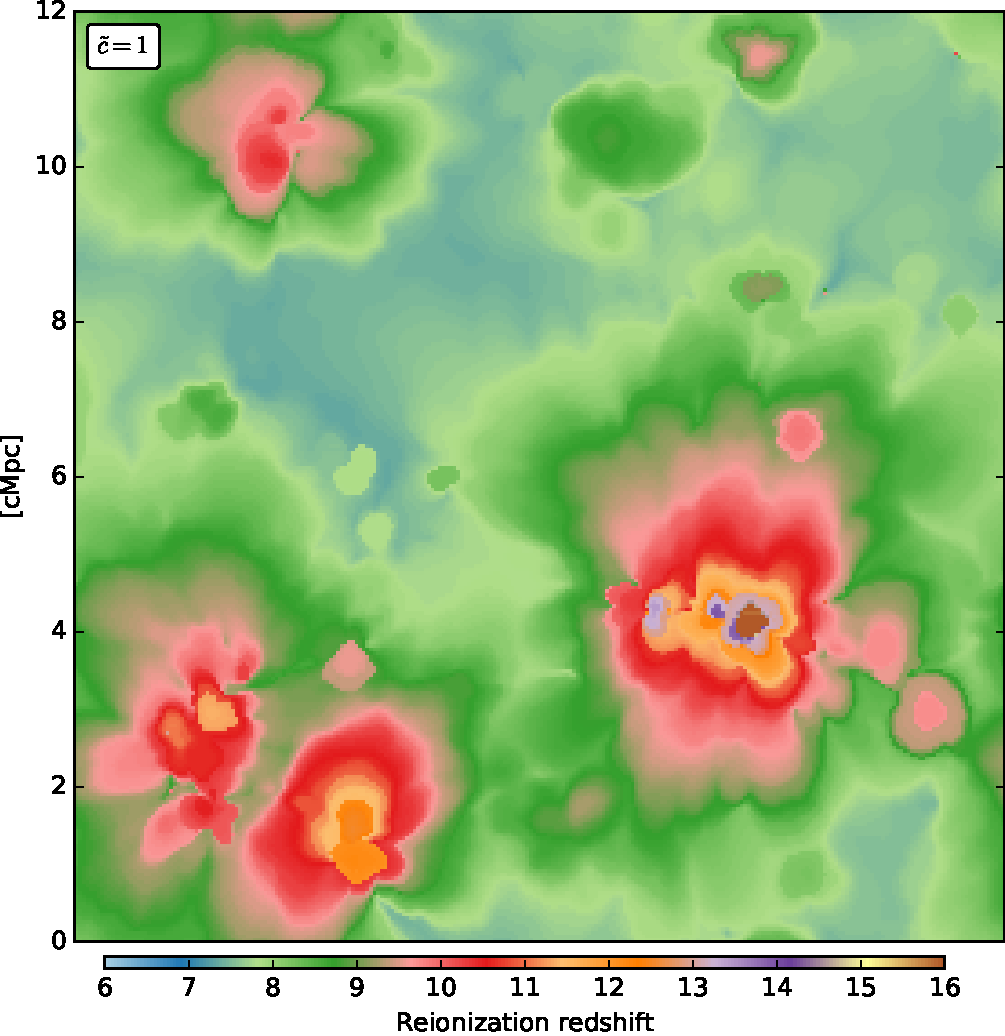
\includegraphics[width=.95\linewidth]{img/04_mapreio/map_z_c1.pdf} 
        \caption{Example de carte de redshift de reionisation généré par EMMA.
        Il s'agit d'une tranche d'une cellule d'épaisseur.
        }
 		\label{fig:zmap}
\end{figure}

\section{Cartes de vitesse d'ionization}

A partir des cartes de redshift de reionisation, il est possible d'annalyser la vitesse de propagation de l'ionisation dans la simulation.
L'idée est la suivante:
En utilisant le fait que les cartes de temps nous donnent un temps pour chaque point de l'espace, il est possible quel est le temps qu'il s'est ecoulé entre la reionisation de deux cellules adjacente, et donc de connaitre la vitesse a laquelle le front d'ionisation les a traversées.

En pratique, la vitesse des fronts sera calculée en calculant le gradient de la carte de temps d'ionisation.
Une fois de plus il est necessaire de travailler avec le temps et non le redshift, ce qui ajoute un argument en faveur du choix de travailler en temps et non en redshift.
De plus en prenant diretement le gradient, on obtient le temps mis par le front pour parcourir une distance dx correspondant a la taille de la cellule.
Il faudra donc prendre l'inverse du gradient pour obtenir une vitesse.

La vitesse des fronts d'ionisation $V_{reio}$ est définis comme :

\begin{equation}
V_{reio}  = \left | \frac{1}{ \vec{\nabla} t_{reio}} \right| .
\end{equation}


Le calcul du gradient etant problèmatique au niveau des interfaces entre niveaux de raffinement, les études présentées ici ont été réalisée en projetant la grille AMR sur le niveau coarse, de manière a n'avoir qu'un seul niveau, et a supprimer ces interfaces.

L'objectif est de comparer la vitesse des fronts d'ionisationa la vitesse de la lumière.
Or il reste un problème a regler, la carte de vitesse obtenue est en unité comobile, alors que la lumière voyage avec une vitesse physique.
Pour contrer ce problème, le gradient devra etre pondéré par la valeur du facteur d'expansion de la cellule associée.
On obtiendra ce facteur par intégration de la cosmologie, de la même facon que pour transformer la carte de temps en carte de redshift.

Au final, le calcul du gradient sera discrétisé de la manière suivante:

\begin{equation}
\vec{\nabla} t_{reio}^i \approx \frac{t^{i+1}  - t^{i-1}}{2a^i \left( x^{i+1}  - x^{i-1} \right)}.
\end{equation}

ou $i$ est l'indice de la cellule, a le facteur d'expansion, $t$ le temps d'ionisation et $x$  la position de la cellule.

Un exemple de carte obtenue est présenté Fig. \ref{fig:vmap}.

\begin{figure}[htpb]
        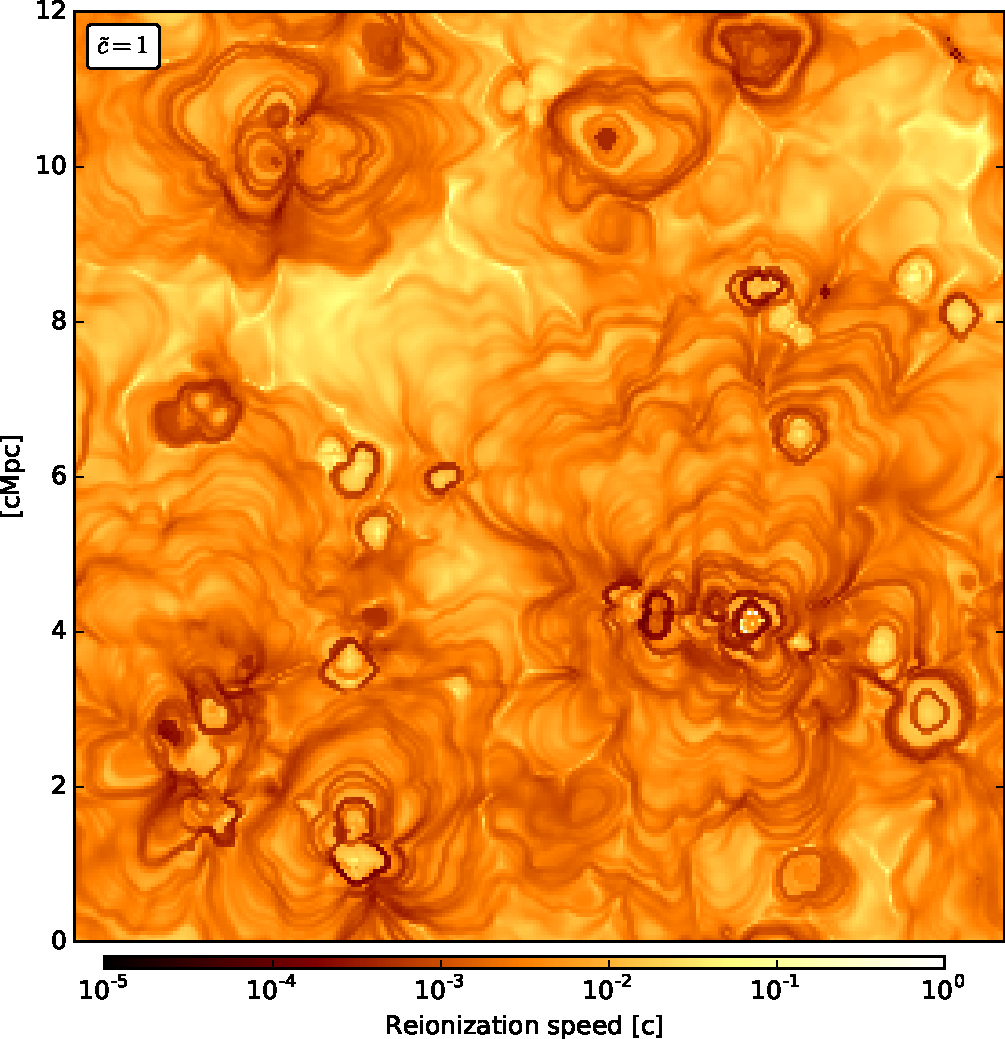
\includegraphics[width=.95\linewidth]{img/04_mapreio/map_v_c1.pdf} 
        \caption{Exemple de carte de vitesse de fronts générée par la méthode du gradient.
		 Cette carte correspond a la même tranche que celle présenté Figure \ref{fig:zmap}
        }
 		\label{fig:vmap}
\end{figure}

TODO DECRIRE LES CARTES\\

\section{vitesse en fonction du redshift}
Nous avons associé a chaque cellule un redshift et une vitesse.
Regardons maintenant comment se comporte l'un par rapport a l'autre sur la Figure. \ref{fig:speedz}.

On observe que la gamme de vitesse est comprise entre 1e-4 et 1e-1 sur une grande partie du processus (avantz=8).
ceci est suivis d'un pic de vitesse puis d'une chute brutale correspondant a l'instant ou toutes les cellules sont reionisées.

\begin{figure}[htpb]
        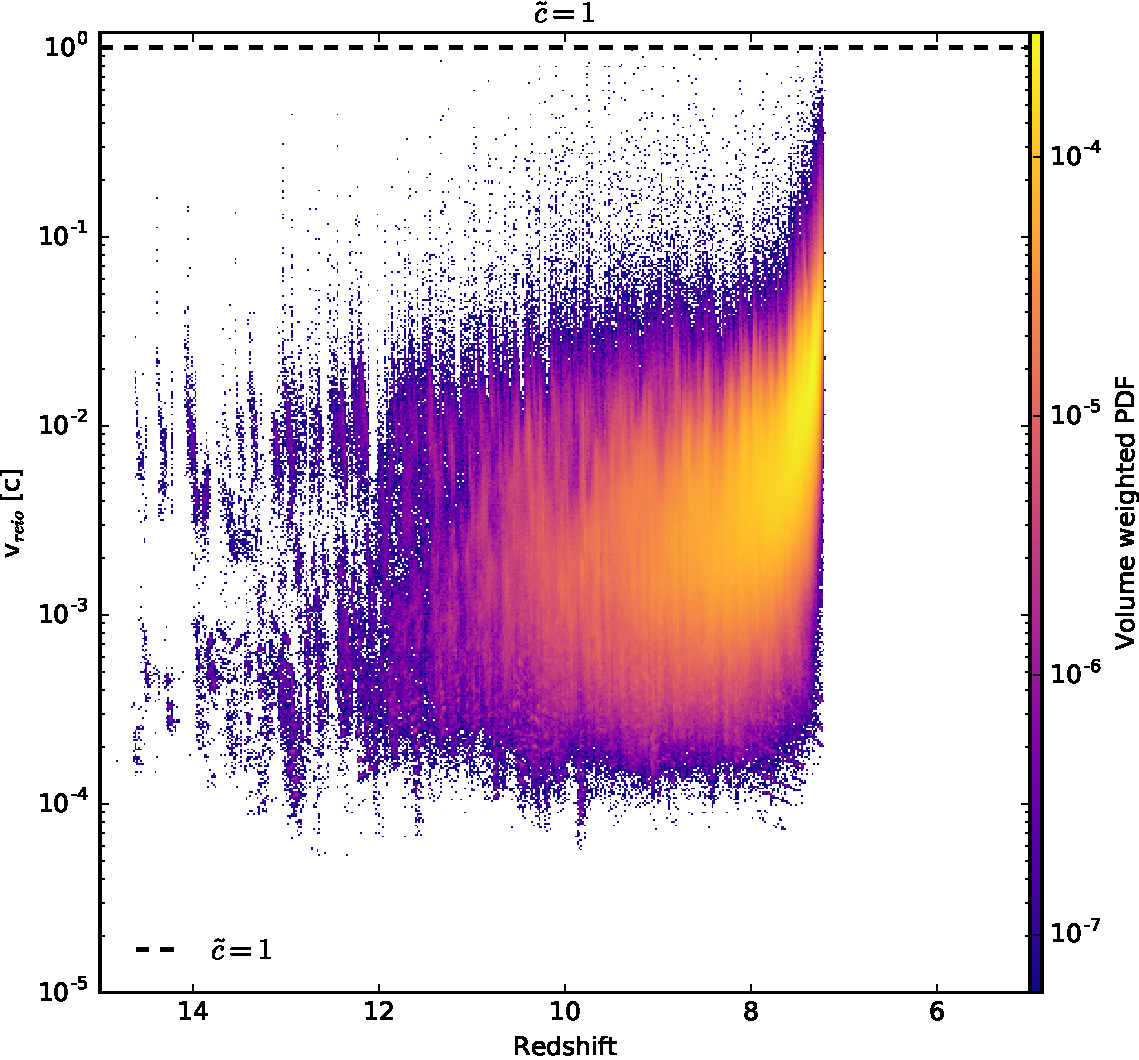
\includegraphics[width=.95\linewidth]{img/04_mapreio/speedreio_z_c1.pdf} 
        \caption{Vitesse d'ionisation en fonction du redshift
        }
 		\label{fig:speedz}
\end{figure}


\section{accélération}
Il est possible de deriver une seconde fois la carte de temps d'ionisation pour obtenir une carte d'accélération des fronts.

\begin{figure}[htpb]
        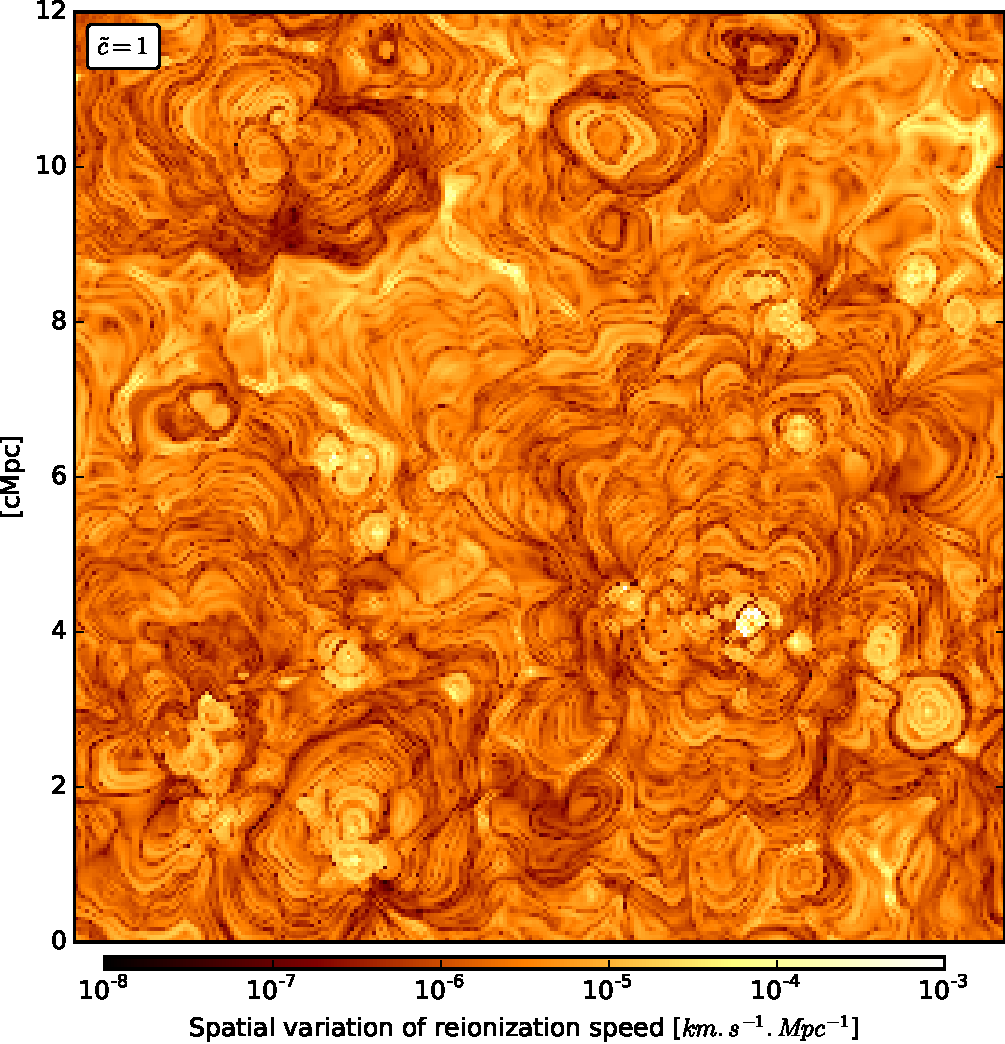
\includegraphics[width=.95\linewidth]{img/04_mapreio/map_acc_c1.pdf} 
        \caption{Vitesse d'ionisation en fonction du redshift
        }
 		\label{fig:speedz}
\end{figure}


